\documentclass[conference]{IEEEtran}
\IEEEoverridecommandlockouts
\usepackage{cite}
\usepackage{amsmath,amssymb,amsfonts}
\usepackage{graphicx}
\usepackage{booktabs}
\usepackage{textcomp}
\usepackage{xcolor}
\usepackage{array}
\usepackage{url}
\usepackage[T1]{fontenc}
\DeclareMathOperator*{\argmax}{arg\,max}
\DeclareMathOperator{\softmax}{softmax}

\begin{document}

\title{DERMA-GUARD: Evidence-Aware Specialist Consensus with Risk-Controlled Evidence Acquisition and Deferral for Multimodal Dermatology}

\author{\IEEEauthorblockN{Rachit Agarwal}
\IEEEauthorblockA{\textit{School of Computer Science and Engineering}\\
\textit{VIT Chennai}, Chennai, India\\
rachit.agarwal2022@vitstudent.ac.in}
\and
\IEEEauthorblockN{Patel Kavya Vipulkumar}
\IEEEauthorblockA{\textit{School of Computer Science and Engineering}\\
\textit{VIT Chennai}, Chennai, India\\
kavya.patel2022@vitstudent.ac.in}
\and
\IEEEauthorblockN{Aarav Prawin}
\IEEEauthorblockA{\textit{School of Computer Science and Engineering}\\
\textit{VIT Chennai}, Chennai, India\\
aarav.prawin2022@vitstudent.ac.in}
\and
\IEEEauthorblockN{Dr. Sindhu Ravindran}
\IEEEauthorblockA{\textit{School of Computer Science and Engineering}\\
\textit{VIT Chennai}, Chennai, India\\
sindhu.ravindran@vit.ac.in}}

\maketitle

\begin{abstract}
Most skin-lesion classifiers do not fail because they are inaccurate on clean benchmark images. They fail because they give every case the same air of confidence: a blurred photograph, a missing history, or a photograph and a history that point to different diagnoses all still produce a label. This paper describes DERMA-GUARD, a decision-support system that picks one of four outcomes instead: a high-confidence answer, a request for more evidence (a dermoscopic image, missing patient details or a better photograph), a plainly marked low-confidence answer that a clinician must confirm, and a referral when the evidence contradicts itself. Six specialists (evidential heads for the photograph, dermoscopy and patient details, an external legacy model, a nearest-neighbour vote and a class-balanced embedding classifier) are profiled case by case by an evidence manager, and a learned gate decides how much each one counts. The gate was selected among seven combination rules by five-fold cross-fitting. A calibrated, cost-aware policy with a Learn-then-Test bound on missed cancers makes the final choice. On 787 held-out MILK10k lesions, 89.1\% of patients receive an answer and 57.1\% receive a high-confidence one that is 77.1\% accurate over eleven diagnoses and misses 3.1\% of cancers, against 4.9\% for a learned rejector ($p=0.011$) and 3.8\% for confidence thresholding at the same coverage. Across four fusion back-ends the policy's miss rate stays between 3.0\% and 3.5\%, whereas thresholding ranges from 3.5\% to 9.3\%. Controlled image damage shows that evidential uncertainty misses blur, darkness, noise and occlusion, while explicit checks remove every confident answer on damaged input. Without retraining, the system stays within its safety target on PAD-UFES-20 and Derm7pt, although its fine-grained diagnosis does not transfer. Re-scoring the earlier prototype, which reported 84--90\%, puts its models at 57--75\% on unseen patients.
\end{abstract}

\begin{IEEEkeywords}
dermatology, multimodal fusion, evidential deep learning, selective prediction, conformal prediction, risk control, evidence acquisition, clinical decision support
\end{IEEEkeywords}

\section{Introduction}
Someone who photographs a mole and asks an app whether it is dangerous almost always gets an answer. It arrives with a number, frequently above 90\%, and the number looks the same whether the photograph was sharp or blurred, whether the person's age and the lesion's site fit the picture, and whether the lesion resembles anything the model was trained on. Deep networks matched dermatologists on curated images several years ago \cite{r1}, so raw accuracy on a benchmark is no longer what limits safe use. Behaviour is.

A careful dermatologist acts differently. With clear evidence they name a diagnosis. Without it they examine the lesion more closely with a dermatoscope, offer a provisional opinion and ask for confirmation, or refer the patient when the history and the lesion disagree. We set out to find whether a model can be built to act in this way and what that costs.

This is our second attempt. The first version of DERMA-GUARD already contained the right ideas: a panel of specialist models, a sceptical component that questions their evidence, and trust that depends on the suspected diagnosis. Its weights, however, were typed in by hand. When we audited it, the accuracies it reported did not hold up. The split had been made by photograph and not by patient, and the evaluation code shifted predictions toward preset accuracy targets (Section~\ref{sec:proto}). We kept the ideas, replaced every hand-set number with one fitted on validation data, and turned each result into a script that can be run again.

Two base papers frame the work (Section~\ref{sec:related}). HOT AI \cite{r2} is the closest in task and asks for a dermoscopic image when the photograph is not enough; Learn-then-Test \cite{r3} supplies the statistical guarantee. We compare against both, or against a faithful baseline derived from them, using the same probabilities.

\textbf{Contributions.}
(i)~A team of six specialists whose per-case weights are learned from all of the evidence manager's signals, selected among seven rules by cross-fitted validation, with an exhaustive subset study and an oracle ceiling.
(ii)~A calibrated four-outcome policy that can ask for three kinds of missing evidence and certifies the missed-cancer rate of its confident answers.
(iii)~The observation that abstention by confidence is only as safe as the fusion beneath it, whereas the calibrated policy stays stable across fusion back-ends.
(iv)~A controlled degradation benchmark, two external tests without retraining, and an honest re-evaluation of the earlier prototype's seven models.
(v)~A working care platform with a web portal for patients, doctors and administrators (Section~\ref{sec:platform}).

\section{Base Papers and Related Work}
\label{sec:related}
\textbf{Base paper 1: HOT AI \cite{r2}.} From a clinical photograph, HOT AI produces a hierarchical diagnosis, an out-of-distribution alert and a recommendation to take a dermoscopic image when the photograph alone is not sufficient; it then fuses both images. It shows that asking for dermoscopy is not a new idea. DERMA-GUARD adds an explicit price for acquiring and for deferring, a separate defer action for contradictory evidence, a certified bound on missed cancers, and stress tests on a public paired dataset. HOT AI's model and data are not public, so we compare against a rule built in its spirit: send the most uncertain patients for dermoscopy, at the same rate as our policy, using the same probabilities.

\textbf{Base paper 2: Learn-then-Test \cite{r3}.} The method selects decision thresholds on held-out data so that a chosen risk is bounded, with a finite-sample guarantee, when future cases resemble the calibration cases. We use it as published for the risk that matters here, the share of answered cancers called benign, inside a three-action policy, and we measure what happens to the guarantee on two other datasets.

\textbf{Data and evaluation.} MILK10k \cite{r4} pairs a clinical close-up with a dermoscopic image for every lesion. A reader study on it \cite{r5} found that dermoscopy is more sensitive for malignancy and the close-up more specific, each adding value; this is the clinical argument for requesting dermoscopy selectively. JI-ADF \cite{r6} reports multimodal fusion on the hidden MILK10k test set, which we did not use, so its numbers cannot be compared with ours. Abstention is scored with AUGRC \cite{r7} and with comparisons at matched coverage, and acquisition against random and oracle bounds in the manner of CAMA \cite{r8}.

\textbf{Classification and fusion.} Networks reached dermatologist level on curated images \cite{r1}, usually on residual architectures \cite{r9}, and dermatology foundation models \cite{r10} are the current frontier. Multimodal work fuses images with metadata \cite{r11} or pairs clinical and dermoscopic images \cite{r12}; PAD-UFES-20 \cite{r13} supplies smartphone photographs with clinical metadata. These models improve the prediction a policy rests on; in this paper fusion is a component and not the contribution.

\textbf{Uncertainty, conformal sets and deferral.} Evidential deep learning \cite{r14} and Dempster--Shafer fusion \cite{r15,r16} give per-case ignorance and conflict, while temperature scaling \cite{r17}, isotonic regression \cite{r18} and Mahalanobis scores \cite{r19} calibrate and flag unusual inputs. Conformal prediction has been validated for skin lesions \cite{r20}, made group-conditional by skin type \cite{r21}, and is smallest on average in its least-ambiguous form \cite{r22}. Chow's rule \cite{r23}, selective classification \cite{r24} and learning to defer \cite{r25} decide when to withhold an answer. Each ingredient exists. The open question is whether a cost model, a statistical guarantee, a three-action policy and combined-failure testing on public paired data together help in measurable ways.

\begin{table*}[!t]
\caption{The two base papers (top) and the other methods compared, with what we measured (MILK10k test, $c_{\mathrm{miss}}=5$).}
\label{tab:base}
\centering\footnotesize
\begin{tabular}{p{2.0cm}p{3.2cm}p{10.2cm}}
\toprule
Work & Its contribution & Our use and measured result \\
\midrule
HOT AI \cite{r2} & asks for dermoscopy when the photograph is insufficient; OOD alert & adds costs, a defer action and a certified bound; HOT-style ``ask the most uncertain'' rule reaches acquisition efficiency $+0.26$ against $+0.07$ for our estimator (it wins), but answering everyone afterwards misses 5.6\% against 3.1\% for our confident answers \\
Learn-then-Test \cite{r3} & risk-controlling thresholds & certified at both stages ($\hat\lambda=0.218,\,0.276$); holds on PAD-UFES-20 (0.0\%) and Derm7pt (3.8\%) \\
Learning to defer \cite{r25} & learned deferral & L2D-style rejector misses 4.9\% against our 3.1\% ($p=0.011$) \\
Confidence threshold \cite{r24} & selective classification & 3.8\% against 3.1\% (n.s.); 3.5--9.3\% across four fusions \\
AUGRC \cite{r7} & abstention metric & ignorance 0.0820 against softmax 0.0757 (softmax better) \\
MILK10k \cite{r4,r5} & paired data; each modality adds value & dermoscopy head AUROC 0.854 against photograph 0.787; fused 0.885 \\
\bottomrule
\end{tabular}
\end{table*}

\section{Data and Evaluation Protocol}
MILK10k \cite{r4} holds 5,240 lesions, each with one clinical close-up and one dermoscopic image, eleven diagnoses (95.7\% confirmed by histopathology; 71.7\% malignant), age, sex, body site, a skin-tone class and seven automatically computed concept scores. Patient identifiers are not provided, so we split by lesion into 3,667 training, 786 validation and 787 test lesions and checked that no lesion appears twice. Everything fitted after the network is fitted on validation: fusion rules, reliabilities, calibration, conformal quantiles, the risk threshold, the acquisition estimator and every choice between methods. The test split was scored once. The classes are heavily imbalanced. Basal cell carcinoma makes up 48\% of lesions, and four classes have fewer than ten test lesions each, which is why macro-F1 and balanced accuracy are reported next to accuracy throughout.

\textbf{External data.} PAD-UFES-20 \cite{r13} (2,298 smartphone photographs, six classes, no dermoscopy) and Derm7pt \cite{r12} (1,003 lesions with both images after mapping its diagnoses onto the MILK10k classes) are used for testing only, with no retraining or recalibration.

\textbf{Metrics.} For a system that may abstain we report coverage (the share of high-confidence answers), accuracy among them, and the missed-cancer rate (the share of answered malignant lesions called benign), always comparing systems at equal coverage. We also report macro-F1 and balanced accuracy for rare classes, malignant-versus-benign AUROC, AUGRC \cite{r7}, and the acquisition efficiency
\begin{equation}
\mathrm{AE}=\frac{G_{\pi}-G_{\mathrm{rand}}}{G_{\mathrm{oracle}}-G_{\mathrm{rand}}}
\label{eq:ae}
\end{equation}
for the choice of whom to send for dermoscopy, where $G$ is the gain obtained by the policy $\pi$, by random selection and by an oracle. Intervals are 95\% bootstrap intervals with paired tests (2,000 resamples).

\section{Method}
Fig.~\ref{fig:arch} shows the pipeline. A case moves from left to right: the specialists give opinions, the evidence manager profiles them, a fusion rule turns the profile into weights, and the policy decides.

\begin{figure*}[!t]
\centering
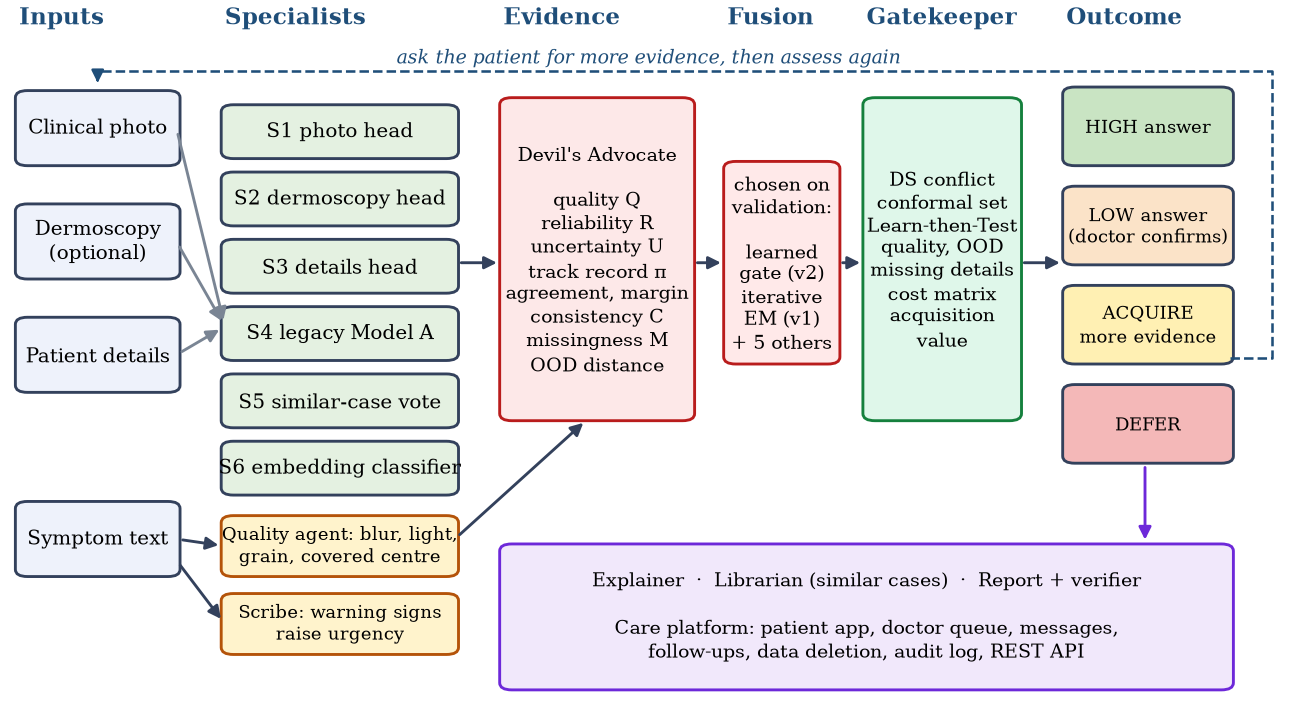
\includegraphics[width=0.86\textwidth]{f_arch.png}
\caption{DERMA-GUARD. Six specialists are profiled by the evidence manager (``Devil's Advocate'') and combined by the fusion rule chosen on validation; the gatekeeper and a cost matrix select one of four outcomes. The dashed loop is the request for more evidence, after which the case is assessed again.}
\label{fig:arch}
\end{figure*}

\subsection{Specialists}
\textbf{S1--S3: evidential heads.} An ImageNet ResNet50 \cite{r9} shared by both image types and a residual metadata network produce three 256-dimensional embeddings. Each embedding feeds an evidential head that outputs non-negative evidence $e_{m}$ \cite{r14}. With $\alpha_{m}=e_{m}+1$ and $S_{m}=\sum_{k}\alpha_{m,k}$, belief and ignorance are
\begin{equation}
b_{m,k}=\frac{e_{m,k}}{S_m},\qquad u_m=\frac{K}{S_m},\qquad p_m=b_m+\frac{u_m}{K}
\label{eq:belief}
\end{equation}
where $p_m$ is the pignistic distribution that a head contributes. Two heads are also combined by Dempster's rule \cite{r16},
\begin{equation}
C=\sum_{i\neq j}b_{1,i}b_{2,j},\quad
b_k=\frac{b_{1,k}b_{2,k}+b_{1,k}u_2+b_{2,k}u_1}{1-C},\quad
u=\frac{u_1u_2}{1-C}
\label{eq:ds}
\end{equation}
which leaves a missing modality ($u=1$) exactly without effect and separates contradiction ($C$) from shared ignorance ($u$). The network was trained on a Kaggle GPU for 25 epochs with modality dropout of 0.25, so that it learns to say ``I don't know'' for an absent input.

\textbf{S4: legacy model.} The image model of the earlier prototype, trained on PAD-UFES-20, is applied as it was. Its six classes are mapped to MILK10k and mixed with 10\% uniform mass, so that unsupported classes are unknown and not impossible.

\textbf{S5, S6: case-based specialists.} S5 is a vote of the 15 most similar training lesions in embedding space, weighted by $\exp(5\,\mathrm{sim})$. S6 is a multinomial logistic regression over all training embeddings with class weights inversely proportional to frequency, so that rare diagnoses are not drowned out; its regularisation was chosen on validation.

\subsection{The evidence manager}
For specialist $m$ on case $x$ the evidence manager computes ten signals. These are the quality $Q_m$ (the share of image statistics that fall inside the training 5th--95th percentiles), a reliability $R_m$ (a logistic regression fitted on validation to predict whether $m$ is right), the normalised entropy $U_m$, the confidence, the margin, the agreement with the other specialists, the measured track record $\pi_m(\hat y_0)=\Pr(m\ \mathrm{correct}\mid y=\hat y_0)$ at the provisional diagnosis, the team's Jensen--Shannon consistency, the missingness, and the Mahalanobis out-of-distribution distance \cite{r19}. The earlier prototype multiplied hand-set versions of these, $E_m=Q_mR_mU_mCSM_m$, and normalised the product into weights. Because the consistency $C$ and the sufficiency $S$ are equal for all specialists of a case, they cancelled, and only three signals ever moved the weights.

\begin{figure}[!t]
\centering
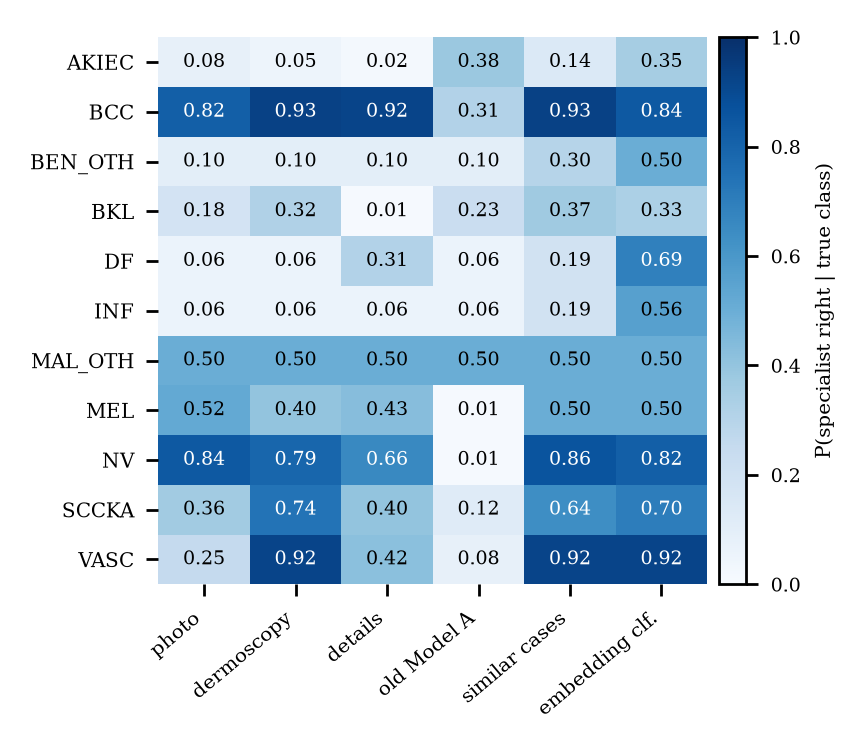
\includegraphics[width=\columnwidth]{f_trust.png}
\caption{The measured trust table $\pi_m(c)$: on validation lesions of each true class, how often each specialist alone names it. The prototype typed this table in by hand; for melanoma it assumed 0.96 for the photograph, where 0.52 is measured.}
\label{fig:trust}
\end{figure}

\subsection{Fusion rules and how one is chosen}
The first rule is an iterative, diagnosis-adaptive fusion (v1) that keeps the prototype's EM-style loop \cite{r26}. Weights $w_m\propto(Q_mR_m)^{a}$ give a provisional diagnosis $\hat y$, and then up to three times
\begin{equation}
w_m=\softmax_m\bigl(a\log Q_mR_m+b\log\pi_m(\hat y)+g\log\kappa_m\bigr)
\label{eq:v1}
\end{equation}
with $\kappa_m=\rho$ for specialists that disagree with $\hat y$, after which the diagnosis is updated.

The learned gate (v2) lets every signal act. With the standardised signal vector $\phi_m(x)$,
\begin{equation}
w_m(x)=\softmax_{m\in\mathrm{present}}\bigl(\beta_m+\theta_m^{\top}\phi_m(x)\bigr)
\label{eq:gate}
\end{equation}
and the opinions are pooled either as a mixture $\sum_m w_mp_m$ or as a product of experts $\propto\prod_m p_m^{w_m}$, followed by temperature scaling. The parameters $\theta$, $\beta$ and the temperature minimise the validation log-loss with an $\ell_2$ penalty.

Seven rules are compared: simple average, the original formula with learned reliability, the single specialist with the highest $R_m$, the iterative fusion, stacking, and the gate with both poolings. Because validation lesions serve twice (to fit the fusion and to calibrate the policy), every rule is cross-fitted: it is fitted on four fifths of validation and applied to the remaining fifth, five times (Fig.~\ref{fig:cf}). The out-of-fold probabilities both select the rule (best macro-F1, fixed before any test result was seen) and calibrate the policy. We also refit the selected rule on all 31 (stage A) and 63 (stage B) specialist subsets, and report an oracle that picks, per case, the specialist giving the true class the most mass.

\begin{figure}[!t]
\centering
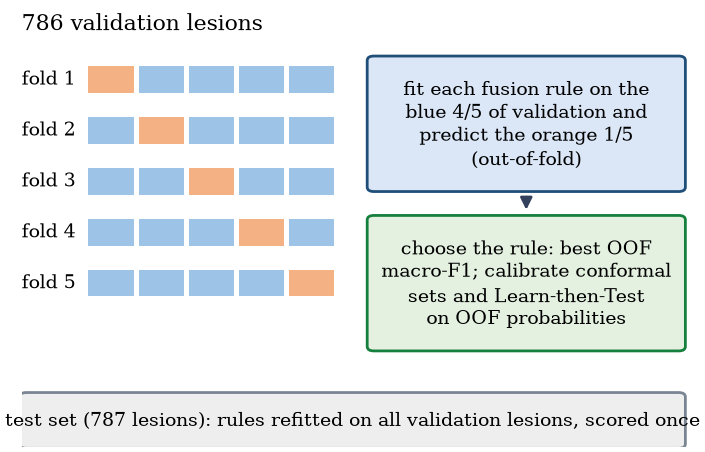
\includegraphics[width=0.92\columnwidth]{f_cf.png}
\caption{Cross-fitting. Every fusion rule is fitted on four validation folds and predicts the fifth; the out-of-fold predictions both choose the rule and calibrate the safety guarantees, so neither step judges a model on its own training data.}
\label{fig:cf}
\end{figure}

\subsection{The decision policy}
Stage A uses the photograph and the patient details, and stage B adds dermoscopy. The stated diagnosis is the most probable class. Costs are 0 for a correct answer, 1 within the benign or the malignant group, $c_{\mathrm{miss}}=5$ for a cancer called benign and 2 for the reverse, with 0.5 to acquire dermoscopy and 1.5 for a clinician review. The gates are the following: Dempster--Shafer conflict above its validation 90th percentile (defer); a Mondrian least-ambiguous conformal set over \{benign, malignant\} ($\alpha=0.1$) \cite{r21,r22} that still contains ``malignant'' when the answer would be benign; a Learn-then-Test threshold \cite{r3} on $1-u$ such that
\begin{equation}
\Pr\bigl(\text{missed-cancer rate}\le 0.05\bigr)\ge 0.9
\label{eq:ltt}
\end{equation}
severe image-quality issues (blur, exposure, contrast, glare, grain or a covered image centre beyond the training 1st/99th percentiles); a Mahalanobis outlier; and missing details (no age, sex or site and no dermoscopy), which triggers a request and not an answer.

If no gate fires and answering is cheapest, the answer is High. Otherwise the system requests dermoscopy when the expected cost after acquisition, estimated by a gradient-boosted regressor fitted on validation lesions whose dermoscopy is known, plus 0.5, is below the cost of review; if not, it gives a Low answer for a clinician to confirm (Fig.~\ref{fig:policy}). Only contradiction or absent evidence leads to a deferral, so the High tier coincides with a conventional defer-on-any-gate policy, and all baseline comparisons concern the same answers. An earlier version deferred on every failed check, which sent each patient without a confident answer to a clinician with nothing at all; the Low tier keeps those patients informed while still requiring confirmation.

\begin{figure}[!t]
\centering
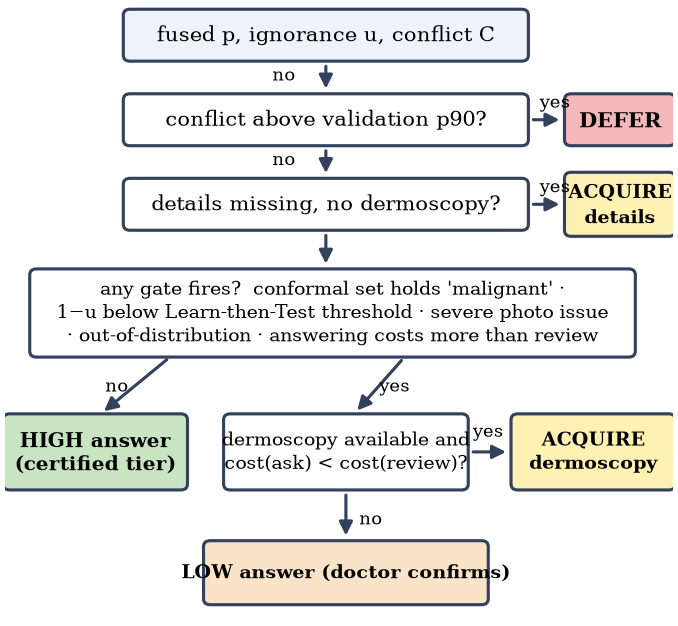
\includegraphics[width=\columnwidth]{f_policy.png}
\caption{How the policy chooses an outcome. Requests for evidence loop back: once the dermoscopic image or the missing details arrive, the case is assessed again.}
\label{fig:policy}
\end{figure}

\subsection{Agents and care platform}
\label{sec:platform}
Around the policy, a quality agent advises on retakes; a scribe raises triage urgency when the patient's own words mention warning signs (with negation handling, and it never changes the diagnosis); a librarian shows similar confirmed training lesions; an explainer states who said what, why dissenting specialists disagree and where the weight went; and a report writer may use a local language model whose output is discarded if a verifier finds any diagnosis or percentage that is not in the evidence. A care platform built on SQLite routes each outcome. A confident answer schedules a follow-up, a request moves the case to ``awaiting patient'' until the evidence arrives, and Low answers and deferrals enter a clinician queue ordered by kind and urgency. A follow-up photograph whose probability of malignancy rises by 0.15 or more returns the case as urgent. Every assessment stores the policy version that produced it, every event goes to an append-only audit log, and patients can delete a case or their whole record, including uploaded photographs. The code base has 230 automated tests.

The platform has a web portal (Figs.~\ref{fig:web1}--\ref{fig:web3}) served by one FastAPI process. A patient registers, uploads a photograph, answers a few questions and receives the result with its evidence; a doctor sees every case, with the images, the specialists' opinions, retrieved similar lesions and agent scores, and records the final decision, which the patient then sees; an administrator sees accounts and the audit log but no clinical content. The portal shown in the figures runs the earlier seven-model prototype of Section~\ref{sec:proto} behind a four-level consensus rule (accept, arbitrate, acquire, escalate), together with the same clinician queue, retrieval of similar documented patients and per-agent scores. The specialist team and the risk-controlled policy of this section are evaluated offline in Section~\ref{sec:results}.

For one held-out melanoma in our test set, the explainer reports that the photograph head named melanoma but was only 10\% sure, that the legacy model said benign keratosis because it ``was trained on a different dataset and cannot name five of the eleven diagnoses'' and was right on only 1\% of validation melanomas, and that most of the weight went to the metadata head, the embedding classifier and the photograph head, which agreed with the team and had high learned reliability for this case. The system then asked for the dermoscopic image. Every number in such an explanation is read from the evidence profile; the language model, when used, may only reword it.

\section{Results}
\label{sec:results}
\subsection{Specialists and fusion}
Table~\ref{tab:spec} summarises the specialists and the fusion rules. Dermoscopy carries real information: the dermoscopy head beats the photograph head on every metric, and adding it lowers the network's mean ignorance from 0.676 to 0.439. The legacy model transfers poorly (21.9\% accuracy). The two case-based specialists are the strongest single sources, and the class-balanced classifier S6 has the best balanced accuracy.

\begin{table}[!t]
\caption{Specialists alone and the main fusion rules on the test split (stage B: with dermoscopy). Val: out-of-fold validation macro-F1 used for selection.}
\label{tab:spec}
\centering\footnotesize
\begin{tabular}{lccccc}
\toprule
 & Val & Acc. & F1 & Bal. & AUROC \\
\midrule
\multicolumn{6}{l}{\emph{Specialists (stage B)}}\\
S1 photograph head & -- & 0.595 & 0.264 & 0.266 & 0.787 \\
S2 dermoscopy head & -- & 0.705 & 0.400 & 0.411 & 0.854 \\
S3 metadata head & -- & 0.600 & 0.246 & 0.252 & 0.749 \\
S4 legacy model & -- & 0.219 & 0.077 & 0.096 & 0.553 \\
S5 nearest-neighbour vote & -- & 0.719 & 0.431 & 0.402 & 0.866 \\
S6 embedding classifier & -- & 0.700 & 0.440 & 0.447 & 0.875 \\
\midrule
\multicolumn{6}{l}{\emph{Fusion, stage A (photograph + details)}}\\
Dempster--Shafer, heads & 0.274 & 0.644 & 0.286 & 0.280 & 0.799 \\
Simple average & 0.344 & 0.637 & 0.343 & 0.338 & 0.824 \\
Iterative EM (v1) & 0.374 & 0.670 & 0.383 & 0.375 & 0.832 \\
Stacking & 0.272 & 0.644 & 0.308 & 0.296 & 0.822 \\
Learned gate (v2)$^\star$ & 0.412 & 0.657 & 0.377 & 0.360 & 0.838 \\
\midrule
\multicolumn{6}{l}{\emph{Fusion, stage B (+ dermoscopy)}}\\
Dempster--Shafer, heads & 0.361 & 0.690 & 0.376 & 0.378 & 0.856 \\
Simple average & 0.457 & 0.714 & 0.422 & 0.400 & 0.870 \\
Iterative EM (v1) & 0.492 & 0.717 & 0.459 & 0.444 & 0.862 \\
Stacking & 0.413 & 0.720 & 0.372 & 0.361 & 0.853 \\
Learned gate (v2)$^\star$ & 0.517 & 0.731 & 0.438 & 0.418 & 0.885 \\
Oracle best specialist & -- & 0.840 & 0.594 & -- & -- \\
\bottomrule
\end{tabular}

\smallskip
\raggedright\scriptsize $^\star$selected (product pooling).
\end{table}

Every way of weighting the team that uses the evidence beats the evidential network alone. Without dermoscopy, macro-F1 rises from 0.286 to 0.377 for the selected gate, and with dermoscopy the gate has the best accuracy (0.731) and AUROC (0.885). The gate won the cross-fitted validation comparison in both stages; on test, the iterative fusion has a slightly higher macro-F1, a reminder that macro-F1 over classes with fewer than ten test lesions is noisy, and we kept the pre-declared choice. Stacking, the textbook learned combiner, is the weakest learned rule: 66 free inputs and 786 validation lesions are not enough for it. Adding S6 raised the selected rule's stage-A macro-F1 from 0.332 to 0.377, and the subset study found no subset that beat the full team by more than 0.033 on validation. The oracle's 0.594 shows that choosing the right specialist per case, and not the specialists themselves, is the bottleneck. On average the gate gives the largest weights to the metadata head (0.35--0.41) and S6 (0.21--0.22), moves weight to dermoscopy when it is present, and gives the legacy model 0.07. Isotonic calibration makes the displayed confidence honest: 0.757 shown on average against 0.731 actual accuracy with dermoscopy, and 0.660 against 0.657 without.

Per class, the team helps most where the evidential network was weakest: benign keratoses (F1 0.16 to 0.51), actinic keratoses (0.24 to 0.47) and the small ``benign other'' and inflammatory classes, which the network never predicted. It is worse on vascular lesions (0.88 to 0.36 on eight test lesions), where the dermoscopy head alone was the best judge, and the single malignant-other lesion is never found.

\subsection{Decisions}
DERMA-GUARD answers 89.1\% of patients (Table~\ref{tab:policy}). Its 57.1\% high-confidence answers are 77.1\% accurate (95\% CI 73.0--80.8\%) and miss 3.1\% of the cancers they answer (1.6--4.8\%); Learn-then-Test certified thresholds at both stages ($\hat\lambda=0.218,\,0.276$). Low-confidence answers are right only 49.6\% of the time, which is why they always go to a clinician, but the truth is within their top three for 85.7\%. Dermoscopy was requested for 29.5\% of patients.

\begin{table}[!t]
\caption{Decision policy and baselines on the same probabilities (test, $c_{\mathrm{miss}}=5$). Abstaining baselines are matched to DERMA-GUARD's coverage.}
\label{tab:policy}
\centering\footnotesize
\begin{tabular}{lccccc}
\toprule
Policy & Ans. & Derm. & Acc. & Missed & Cost \\
\midrule
Always answer, photograph & 100\% & 0\% & 0.657 & 7.2\% & 0.759 \\
Always acquire, answer & 100\% & 100\% & 0.731 & 6.4\% & 1.124 \\
Confidence threshold (B3) & 57.1\% & 0\% & 0.815 & 3.8\% & 0.881 \\
Learned rejector (L2D) & 57.1\% & 0\% & 0.764 & 4.9\% & -- \\
Entropy-chosen acquisition & 100\% & 29.5\% & 0.700 & 5.6\% & 0.790 \\
DERMA-GUARD, High tier & 57.1\% & 29.5\% & 0.771 & 3.1\% & 1.047 \\
\bottomrule
\end{tabular}

\smallskip
\raggedright\scriptsize DERMA-GUARD outcomes: High 57.1\%, Low 32.0\% (top-3 85.7\%), Defer 10.9\%.
\end{table}

At the same coverage, a learned rejector trained to predict the model's own errors \cite{r25} misses 4.9\% of cancers, significantly more than DERMA-GUARD ($+1.8$ points, CI $+0.2$ to $+3.5$, one-sided $p=0.011$). Plain confidence thresholding misses 3.8\%; the difference ($+0.7$ points, CI $-0.7$ to $+2.0$, $p=0.18$) is not significant, and thresholding is more accurate (81.5\% against 77.1\%) because it answers only the photograph's easiest cases. Always answering is cheapest in mean cost, since every clinician review is charged 1.5.

Is the gap to thresholding real? We ran the identical policy on four fusion back-ends (Fig.~\ref{fig:backend}). Its miss rate barely moved, 3.0--3.5\%. The threshold's moved almost threefold, from 3.5\% (the five-specialist gate) to 9.3\% (the five-specialist iterative fusion). A confidence threshold is exactly as safe as the ranking it receives, and nobody deploying it knows in advance which kind of ranking they have; the calibrated policy delivers the same certified rate on all four. The same comparison contains a result against us: the learned acquisition estimator chose whom to send for dermoscopy far better than entropy on the iterative fusion (AE $+0.30$ against $-0.04$) but worse on the final gate ($+0.07$ against $+0.26$), and ignorance ranked errors better than softmax on the former (AUGRC 0.0874 against 0.0918) but not on the latter (0.0820 against 0.0757). Once the fused probabilities are good, simple uncertainty is a good enough guide.

\begin{figure}[!t]
\centering
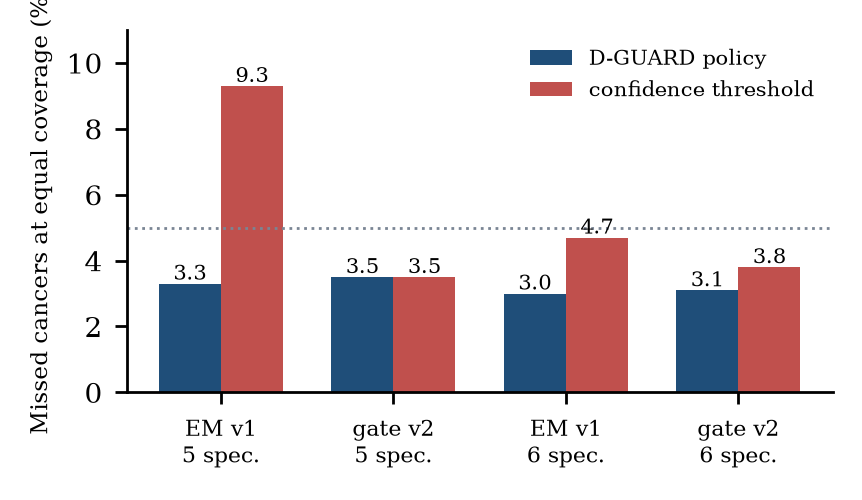
\includegraphics[width=\columnwidth]{f_backend.png}
\caption{The identical policy over four fusion back-ends (iterative EM or learned gate, with five or six specialists). The policy's missed-cancer rate stays at 3.0--3.5\%; confidence thresholding at the same coverage ranges from 3.5\% to 9.3\%.}
\label{fig:backend}
\end{figure}

Raising $c_{\mathrm{miss}}$ from 2 to 10 lowers the High share from 61.6\% to 53.4\% and the miss rate from 4.1\% to 1.9\% (thresholding: 3.8\% at the same coverage), while about 89\% of patients still get an answer. The cost of a missed cancer is therefore a dial that a deploying clinic can set, and not a hidden constant.

Fairness is a weakness: for the 67 test lesions of skin tone 2 the High miss rate is 11.5\%, against 2.2\% for tone 3 ($n=489$); tone 1 has only 14 lesions. MILK10k is dominated by tone 3, and a calibration fitted on the whole validation set guarantees an average and not every group. Group-wise calibration needs more lighter-tone data than the dataset contains.

\subsection{Robustness: DERMA-STRESS}
We damaged the photograph of 300 test lesions in six ways without retraining. Evidential ignorance does not catch what matters. Gaussian blur lowers mean ignorance (0.679 to 0.605) and raises the high-confidence rate (46\% to 50\%), and under-exposed and occluded photographs keep 22\% and 16\% high-confidence answers that miss 12.3\% and 14.3\% of cancers. Explicit checks do catch it: the quality agent flags every blurred, dark, noisy and occluded photograph (the last two through the grain and covered-centre checks), and every case without metadata becomes a request for it. With these checks no damaged input received a high-confidence answer; JPEG artefacts kept 22\% at 1.5\% missed. The price is that 8\% of clean photographs are also flagged.

Read as an ablation, the experiments say the following. Weighting the specialists by their evidence instead of fusing only the evidential heads adds 0.091 photograph-only macro-F1 (0.286 to 0.377), and the sixth specialist alone accounts for 0.045 of it. Cross-fitting removed an optimistic three points of High coverage that in-sample fitting had produced. The calibrated policy, and not any particular fusion, keeps the miss rate at 3.0--3.5\%. The explicit image and missing-details checks, not evidential ignorance, are what remove confident answers on damaged input.

\subsection{External tests}
The calibration guarantees assume that future patients resemble calibration patients. Table~\ref{tab:ext} shows what happens when they do not. On both external datasets, ignorance, quality flags and deferrals rise and the high-confidence share falls from 57\% to 11--13\%. Among the confident answers that remain, the safety target holds: no cancer was missed on PAD-UFES-20 and 3.8\% on Derm7pt, below thresholding's 5.4\%. On Derm7pt, where dermoscopy exists, the system asked for it for 39\% of lesions and overall accuracy rose from 0.402 with photographs alone to 0.479. The eleven-class diagnosis does not transfer: half of PAD-UFES-20's confident answers are wrong, melanoma recall on Derm7pt is 31\%, and thresholding is more accurate on both datasets (Fig.~\ref{fig:ext}). Nothing was retrained on either dataset; they were deliberately kept out of training so that they measure what a deployment would meet.

\begin{table}[!t]
\caption{The MILK10k system on two other datasets, unchanged. Threshold: confidence thresholding at the same coverage.}
\label{tab:ext}
\centering\footnotesize
\begin{tabular}{lccc}
\toprule
 & MILK10k & PAD-UFES-20 & Derm7pt \\
\midrule
Dermoscopy available & yes & no & on request \\
Malignant share & 72\% & 79\% & 29\% \\
Photos failing quality check & 8\% & 28\% & 29\% \\
Dermoscopy requested & 30\% & 28\% & 39\% \\
Accuracy, all cases & 0.731 & 0.367 & 0.479 \\
Malignant AUROC & 0.885 & 0.840 & 0.738 \\
High share & 57.1\% & 11.4\% & 13.0\% \\
Accuracy of High answers & 0.771 & 0.517 & 0.708 \\
Missed cancers, High & 3.1\% & 0.0\% & 3.8\% \\
Threshold: missed / acc. & 3.8\% / 0.815 & 0.0\% / 0.574 & 5.4\% / 0.846 \\
\bottomrule
\end{tabular}
\end{table}

\begin{figure}[!t]
\centering
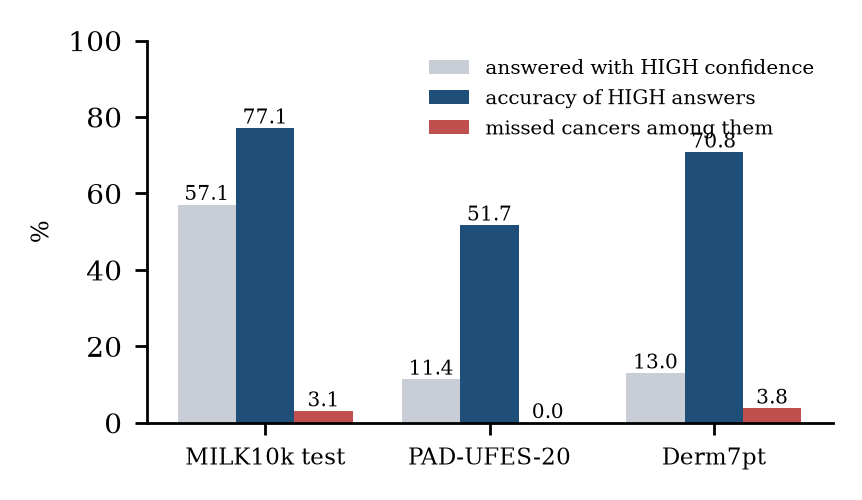
\includegraphics[width=\columnwidth]{f_external.png}
\caption{Share of High answers, their accuracy and the cancers missed among them, on MILK10k and the two external datasets.}
\label{fig:ext}
\end{figure}

\subsection{The earlier prototype, re-evaluated}
\label{sec:proto}
The prototype trained seven PAD-UFES-20 models (image, metadata, free text and their combinations) and reported 84--90\% accuracy. Its split was random by photograph, so 43\% of test photographs came from a lesion and 62\% from a patient already in training, and its evaluation function swapped probabilities between the true class and its closest rival until the number of correct predictions met a hard-coded target for each model. We loaded the saved weights and cached features unchanged and scored them honestly (Table~\ref{tab:proto}, Fig.~\ref{fig:proto}). On the 132 test photographs of unseen patients the image model reaches 56.8\%, the metadata model 75.0\%, the text model (whose ``narratives'' were generated from the metadata) 27.3\%, and the three-modality model 57.6\%, worse than metadata alone. Fusing the seven with our learned gate, cross-validated on those 132 photographs, gives 72.7\% against 59.8\% for averaging them; the gate recovers almost all of the best model's accuracy without being told which model that is.

\begin{table}[!t]
\caption{The prototype's models on PAD-UFES-20: reported accuracy and honest re-scoring of the same saved weights.}
\label{tab:proto}
\centering\footnotesize
\begin{tabular}{llccc}
\toprule
 & Inputs & Reported & Same test & Unseen patients \\
\midrule
A & image & 85.5\% & 61.4\% & 56.8\% \\
B & metadata & 84.1\% & 75.9\% & 75.0\% \\
C & free text & 83.5\% & 23.5\% & 27.3\% \\
D & image + metadata & 88.4\% & 63.5\% & 58.3\% \\
E & image + text & 88.1\% & 61.4\% & 57.6\% \\
F & text + metadata & 87.2\% & 72.2\% & 72.7\% \\
G & all three & 89.9\% & 62.0\% & 57.6\% \\
\midrule
\multicolumn{4}{l}{A--G fused by the learned gate (unseen patients)} & 72.7\% \\
\multicolumn{4}{l}{A--G simple average (unseen patients)} & 59.8\% \\
\bottomrule
\end{tabular}
\end{table}

\begin{figure}[!t]
\centering
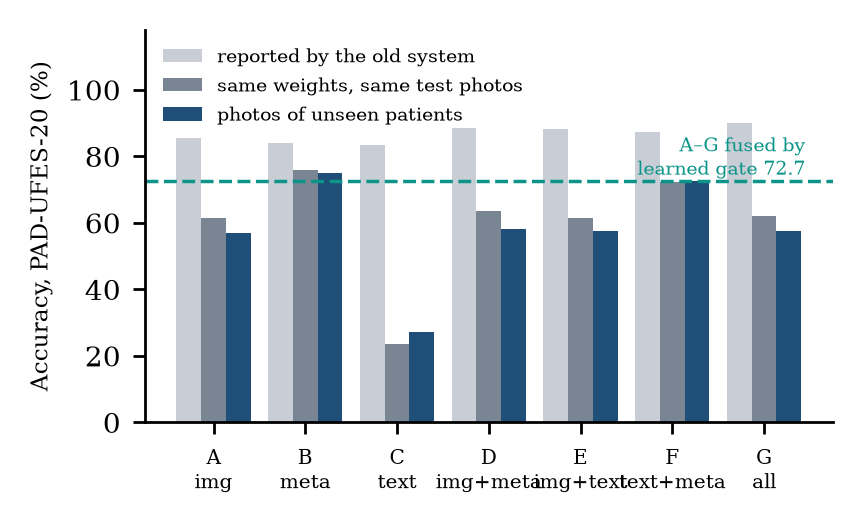
\includegraphics[width=\columnwidth]{f_proto.png}
\caption{The earlier prototype's seven PAD-UFES-20 models: accuracy as reported, re-scored with the same weights on the same test photographs, and on photographs of patients never seen in training. Dashed: the seven fused by the learned gate (cross-validated).}
\label{fig:proto}
\end{figure}

Finally, the PAD-UFES-20 questionnaire lets us test the scribe's triage rule. Of 1,641 lesions, those with any of its warning signs were malignant (BCC, SCC or melanoma) in 48.7\% of cases against 12.4\% without (relative risk 3.9, 95\% CI 2.8--5.5), and every single sign had a relative risk between 1.65 and 3.0. A raised lesion, which the scribe did not originally look for, carried a relative risk of 2.8 and was added as a result. These are clinician-collected questionnaire answers and not free text, so the analysis supports the direction of the rule, not its exact wording.

\begin{figure*}[!t]
\centering
\begin{minipage}[t]{0.49\textwidth}
\centering
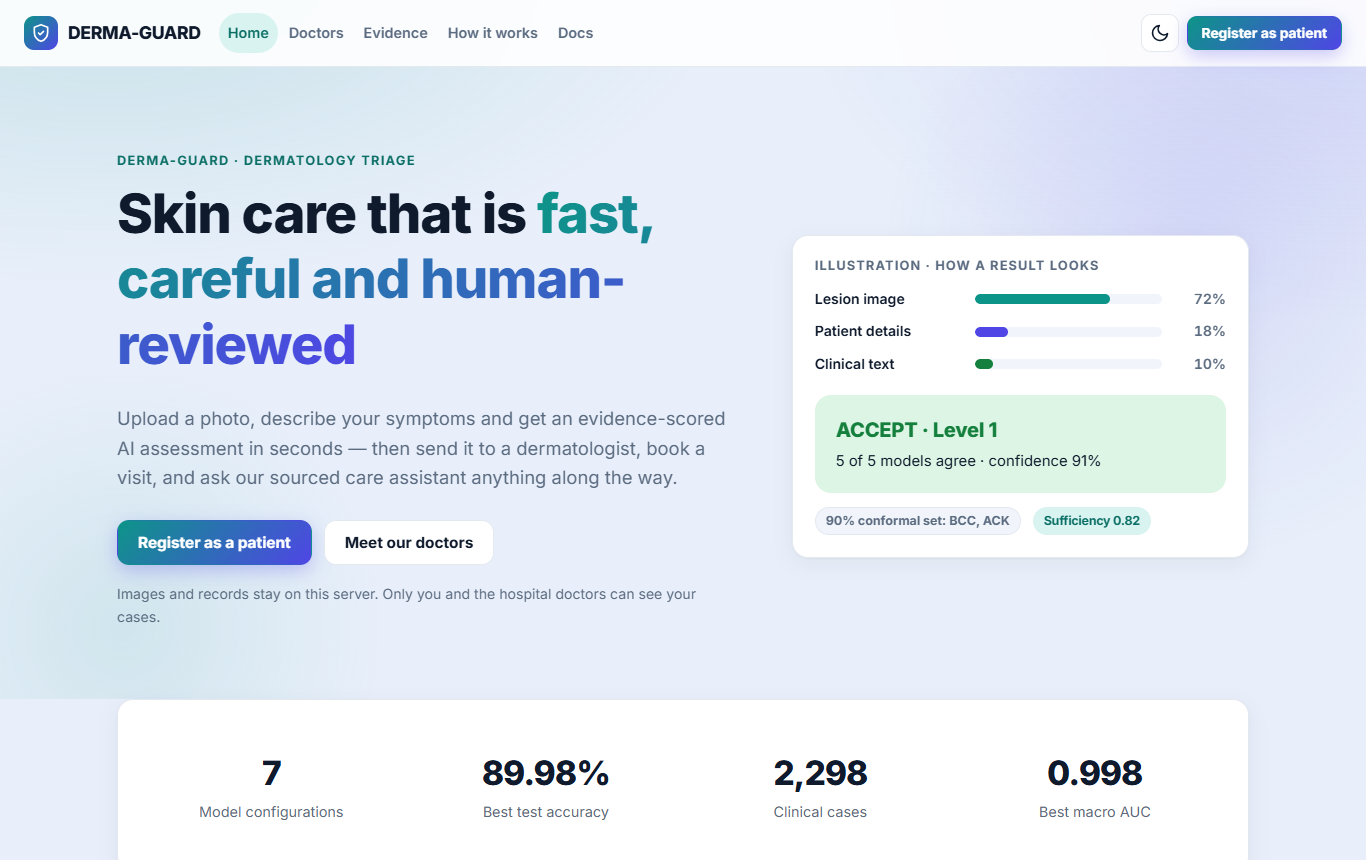
\includegraphics[width=\textwidth]{web_home.png}
\end{minipage}\hfill
\begin{minipage}[t]{0.49\textwidth}
\centering
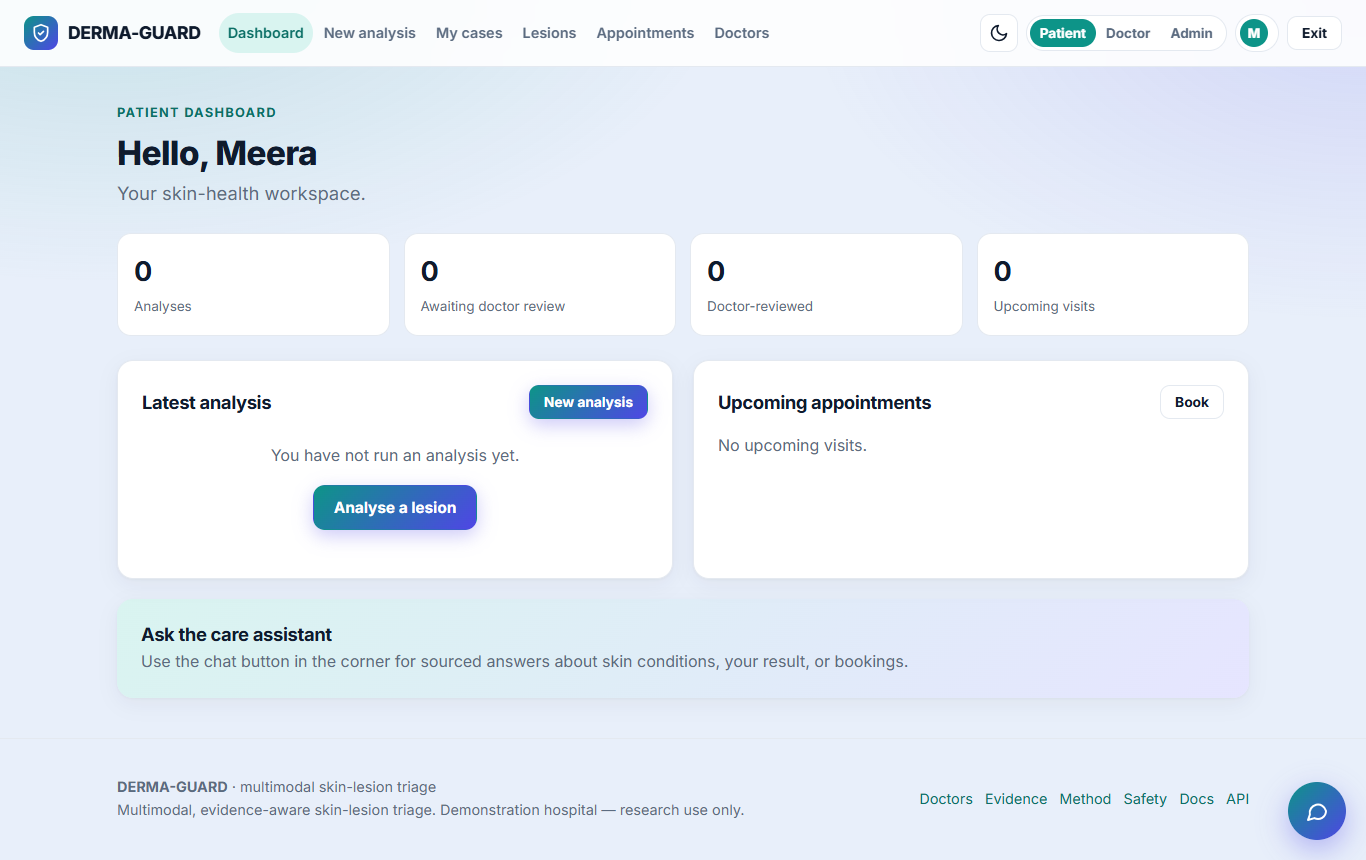
\includegraphics[width=\textwidth]{web_dashboard.png}
\end{minipage}
\caption{The DERMA-GUARD web portal. Left: landing page with the benchmark summary and the registration entry. Right: the patient dashboard after registration, showing the Patient / Doctor / Admin switch used to review a case.}
\label{fig:web1}
\end{figure*}

\begin{figure*}[!t]
\centering
\begin{minipage}[t]{0.40\textwidth}
\centering
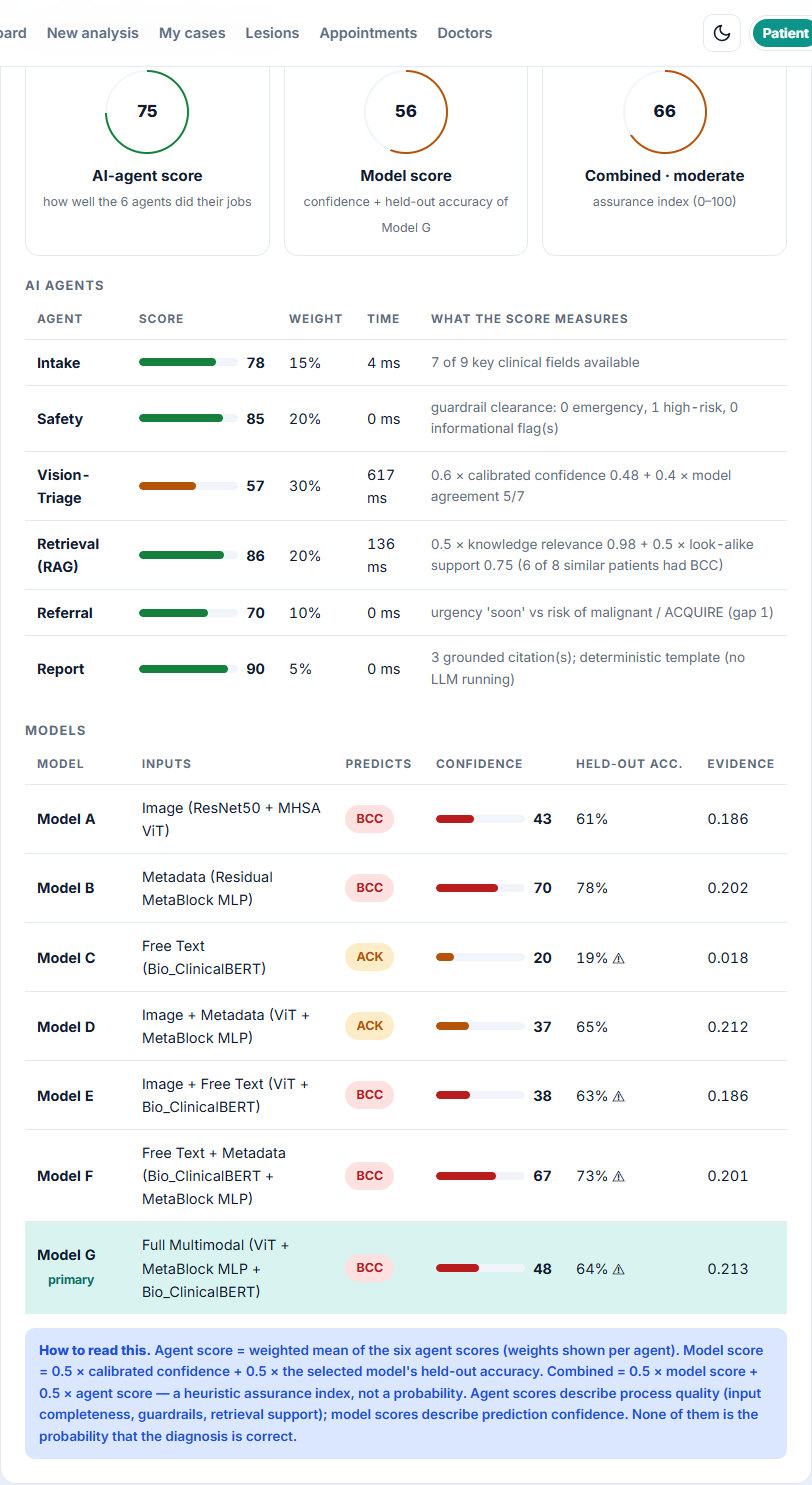
\includegraphics[width=\textwidth]{web_scores.png}
\end{minipage}\hfill
\begin{minipage}[t]{0.57\textwidth}
\centering
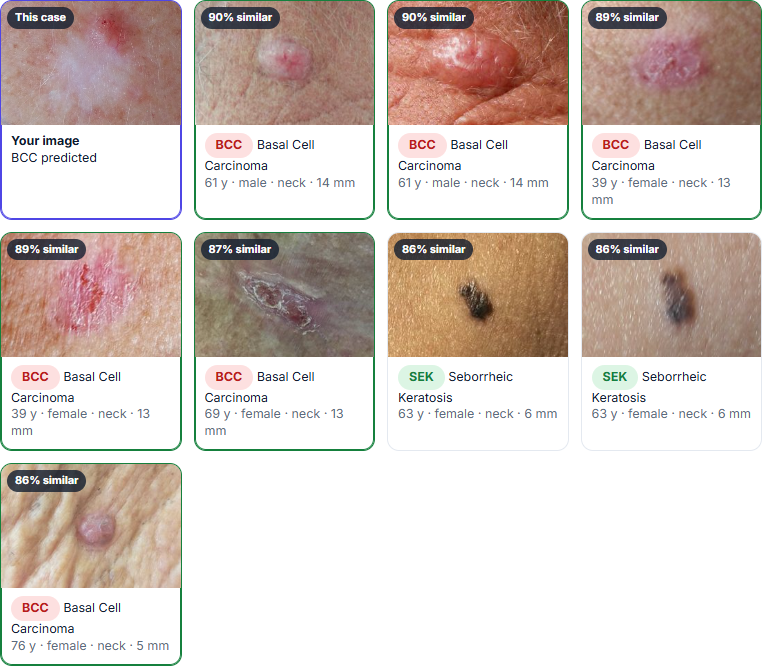
\includegraphics[width=\textwidth]{web_rag.png}
\end{minipage}
\caption{The patient's case view. Left: the score panel with an agent score, a model score and a combined index, followed by the per-agent table with the basis of each score. Right: retrieval of the most similar documented patients, shown beside the patient's own photograph, with green outlines for lesions that share the model's top class.}
\label{fig:web2}
\end{figure*}

\begin{figure*}[!t]
\centering
\begin{minipage}[t]{0.49\textwidth}
\centering
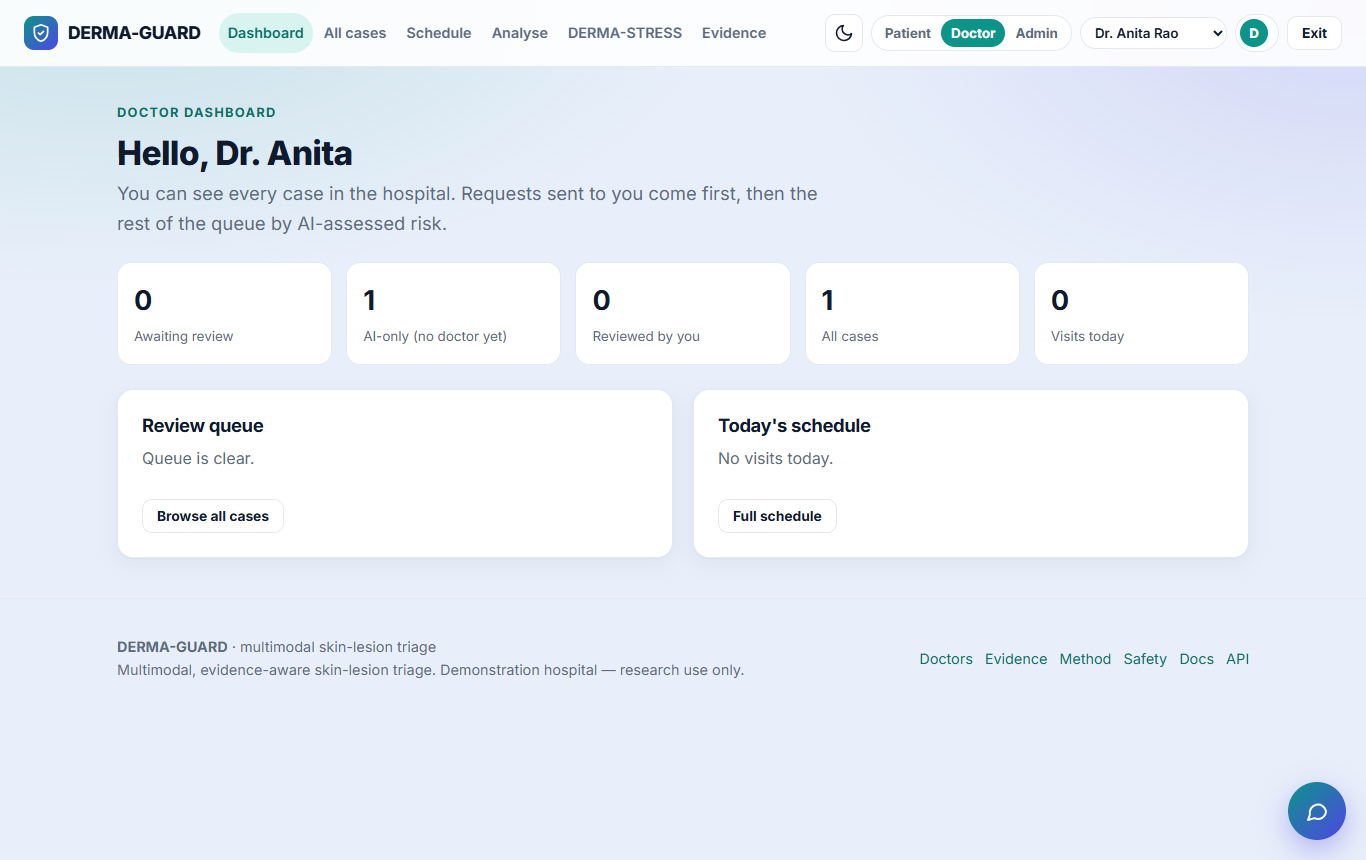
\includegraphics[width=\textwidth]{web_doctor_dashboard.png}
\end{minipage}\hfill
\begin{minipage}[t]{0.49\textwidth}
\centering
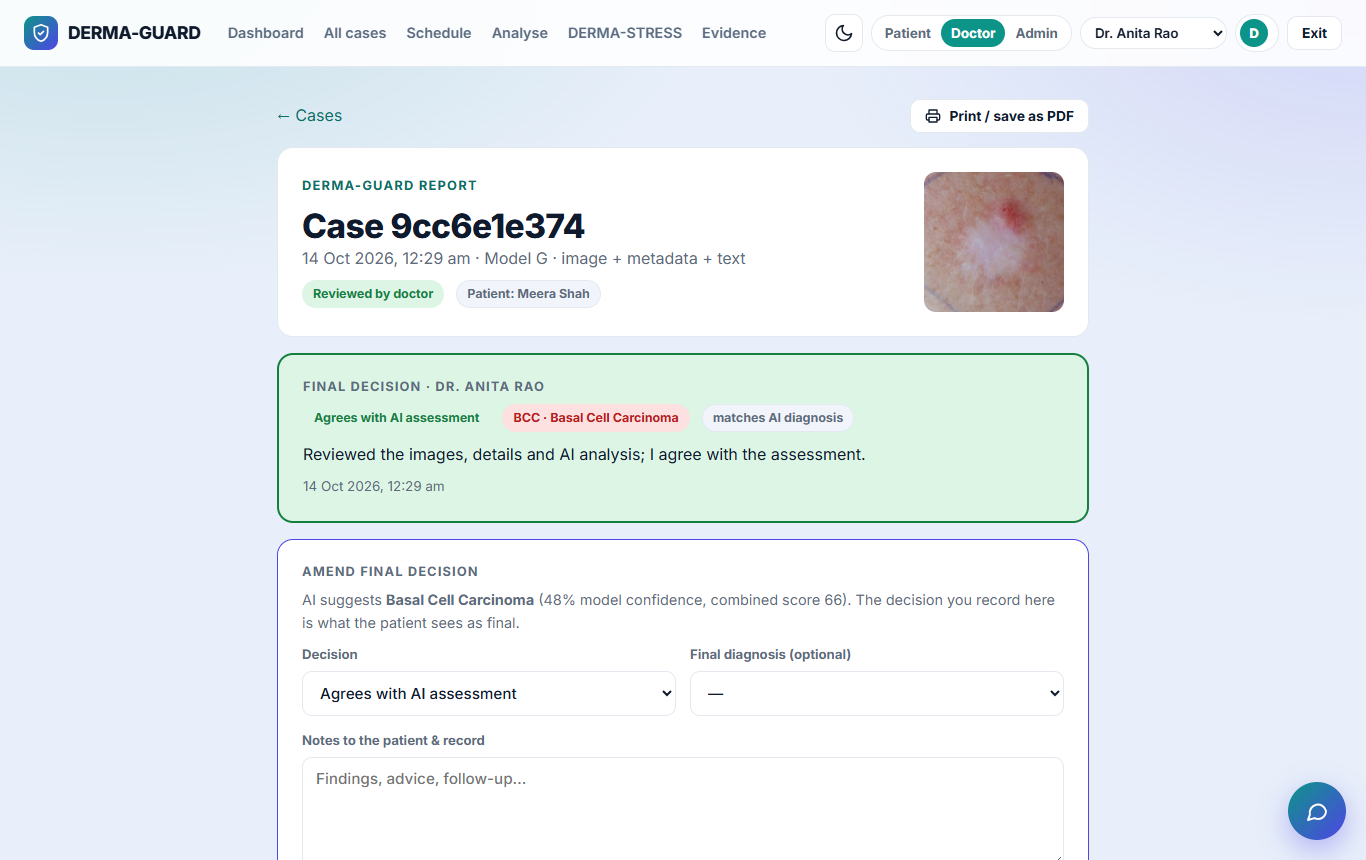
\includegraphics[width=\textwidth]{web_final_decision.png}
\end{minipage}
\caption{The clinician workflow. Left: the doctor dashboard with the review queue of every case in the hospital. Right: the final-decision card shown once the doctor has recorded a decision on the case.}
\label{fig:web3}
\end{figure*}

\section{Discussion}
\textbf{What the earlier design got right.} Consulting several specialists, questioning their evidence and trusting them according to the suspected diagnosis all survived honest evaluation. Every evidence-aware rule beat both the evidential network alone and plain averaging, and the measured trust table (Fig.~\ref{fig:trust}) confirms clinical intuition: dermoscopy is reliable for squamous lesions and the photograph for melanoma. What the earlier design got wrong was its evidence.

\textbf{What did not work.} Stating the minimum-cost diagnosis (classic Chow \cite{r23}) labelled 98.5\% of lesions malignant on this 72\%-malignant population. Adaptive prediction sets for the safety gate collapsed to the full set and deferred every patient. Post-hoc logit adjustment raised validation macro-F1 from 0.36 to 0.44 but lowered test macro-F1 from 0.376 to 0.359. Fitting the fusion in-sample on the calibration lesions inflated the high-confidence share by three points before cross-fitting. Classes with fewer than ten test lesions are almost never predicted.

\textbf{Where the gain comes from.} The oracle that picks the best specialist per case reaches 0.594 macro-F1, against 0.438 for the learned gate. The specialists already hold much of the right answer, and deciding whom to believe is the hard part. A gate trained on more validation data, or distilled from the oracle, is the most direct way forward, and a dermatology foundation backbone \cite{r10} would lift every specialist.

\textbf{Lessons about evaluation.} Split by the unit you will meet in practice; never post-process predictions with the label; choose on validation and keep the choice when the test disagrees; and compare against simple baselines on the same probabilities, and on more than one model. The most useful finding of this work, that thresholding's safety is borrowed from the fusion beneath it, appears only under that last rule.

\textbf{Limitations.} All results come from one training seed of an ImageNet ResNet50; 786 validation lesions do a great deal of fitting; MILK10k is a referral population without patient or centre identifiers; the costs are declared and not derived; the guarantees assume exchangeability; the image checks are heuristics; lighter skin tones are under-served; and the system has not been evaluated in a clinic. The web portal runs the earlier seven-model prototype, and passwordless registration and role switching are demonstration conveniences that must be replaced before use with real patient data.

\section{Conclusion}
DERMA-GUARD turns a team of imperfect specialists into calibrated clinical actions. It answers nine in ten patients, more than half of them with a confident answer that misses about one cancer in thirty, asks for dermoscopy, details or a better photograph when these are needed, and refers only when the evidence contradicts itself. Learning how much to trust each specialist from all of its evidence improves photograph-only diagnosis by a third. The calibrated policy is safer than a learned rejector and, unlike confidence thresholding, remains safe whichever fusion it is given. The lesson we would most like to pass on is methodological: report the simple baseline on the same probabilities, on more than one model, and keep every number reproducible.

\section*{Reproducibility}
Code, per-case predictions and the script behind every table and figure are in the project repository. Model weights and images are not redistributed; MILK10k is available from the ISIC Archive under CC-BY-NC.

\begin{thebibliography}{00}
\bibitem{r1} A. Esteva, B. Kuprel, R. A. Novoa, J. Ko, S. M. Swetter, H. M. Blau, and S. Thrun, ``Dermatologist-level classification of skin cancer with deep neural networks,'' \textit{Nature}, vol. 542, pp. 115--118, 2017.
\bibitem{r2} D. Mehta \textit{et al.}, ``Multi-task AI models in dermatology: Overcoming critical clinical translation challenges for enhanced skin lesion diagnosis,'' \textit{J. Eur. Acad. Dermatol. Venereol.}, vol. 39, no. 12, pp. 2121--2133, 2025.
\bibitem{r3} A. N. Angelopoulos, S. Bates, E. J. Cand\`es, M. I. Jordan, and L. Lei, ``Learn then test: Calibrating predictive algorithms to achieve risk control,'' \textit{Ann. Appl. Stat.}, 2025, arXiv:2110.01052.
\bibitem{r4} MILK study team, ``MILK10k: Multimodal imaging of lesions with knowledge,'' International Skin Imaging Collaboration (ISIC) Archive, 2025, CC-BY-NC.
\bibitem{r5} C. M\"uller \textit{et al.}, ``Comparative and complementary diagnostic value of dermatoscopy and clinical close-up photography in skin cancer diagnosis: A study from the MILK10k dataset,'' \textit{J. Am. Acad. Dermatol.}, 2026.
\bibitem{r6} JI-ADF authors, ``JI-ADF: Joint-individual learning with adaptive decision fusion for multimodal skin lesion classification,'' arXiv:2604.27343, 2026.
\bibitem{r7} J. Traub \textit{et al.}, ``Overcoming common flaws in the evaluation of selective classification systems,'' in \textit{Proc. NeurIPS}, 2024, arXiv:2407.01032.
\bibitem{r8} T. Rheude \textit{et al.}, ``Cohort-based active modality acquisition,'' arXiv:2505.16791, 2025.
\bibitem{r9} K. He, X. Zhang, S. Ren, and J. Sun, ``Deep residual learning for image recognition,'' in \textit{Proc. IEEE CVPR}, 2016, pp. 770--778.
\bibitem{r10} S. Yan \textit{et al.}, ``A multimodal vision foundation model for clinical dermatology,'' \textit{Nature Medicine}, 2025, arXiv:2410.15038.
\bibitem{r11} A. G. C. Pacheco and R. A. Krohling, ``An attention-based mechanism to combine images and metadata in deep learning models applied to skin cancer classification,'' \textit{IEEE J. Biomed. Health Inform.}, vol. 25, no. 9, pp. 3554--3563, 2021.
\bibitem{r12} J. Kawahara, S. Daneshvar, G. Argenziano, and G. Hamarneh, ``Seven-point checklist and skin lesion classification using multitask multimodal neural nets,'' \textit{IEEE J. Biomed. Health Inform.}, vol. 23, no. 2, pp. 538--546, 2019.
\bibitem{r13} A. G. C. Pacheco \textit{et al.}, ``PAD-UFES-20: A skin lesion dataset composed of patient data and clinical images collected from smartphones,'' \textit{Data in Brief}, vol. 32, p. 106221, 2020.
\bibitem{r14} M. Sensoy, L. Kaplan, and M. Kandemir, ``Evidential deep learning to quantify classification uncertainty,'' in \textit{Proc. NeurIPS}, 2018, pp. 3179--3189.
\bibitem{r15} G. Shafer, \textit{A Mathematical Theory of Evidence}. Princeton, NJ, USA: Princeton Univ. Press, 1976.
\bibitem{r16} Z. Han, C. Zhang, H. Fu, and J. T. Zhou, ``Trusted multi-view classification,'' in \textit{Proc. ICLR}, 2021, arXiv:2102.02051.
\bibitem{r17} C. Guo, G. Pleiss, Y. Sun, and K. Q. Weinberger, ``On calibration of modern neural networks,'' in \textit{Proc. ICML}, 2017.
\bibitem{r18} B. Zadrozny and C. Elkan, ``Transforming classifier scores into accurate multiclass probability estimates,'' in \textit{Proc. ACM SIGKDD}, 2002.
\bibitem{r19} K. Lee, K. Lee, H. Lee, and J. Shin, ``A simple unified framework for detecting out-of-distribution samples and adversarial attacks,'' in \textit{Proc. NeurIPS}, 2018.
\bibitem{r20} J. Fayyad \textit{et al.}, ``Empirical validation of conformal prediction for trustworthy skin lesions classification,'' \textit{Comput. Methods Programs Biomed.}, 2024.
\bibitem{r21} C. Lu, A. Lemay, K. Chang, K. H\"obel, and J. Kalpathy-Cramer, ``Fair conformal predictors for applications in medical imaging,'' in \textit{Proc. AAAI}, 2022, arXiv:2109.04392.
\bibitem{r22} M. Sadinle, J. Lei, and L. Wasserman, ``Least ambiguous set-valued classifiers with bounded error levels,'' \textit{J. Am. Stat. Assoc.}, vol. 114, no. 525, pp. 223--234, 2019.
\bibitem{r23} C. K. Chow, ``On optimum recognition error and reject tradeoff,'' \textit{IEEE Trans. Inf. Theory}, vol. 16, no. 1, pp. 41--46, 1970.
\bibitem{r24} Y. Geifman and R. El-Yaniv, ``Selective classification for deep neural networks,'' in \textit{Proc. NeurIPS}, 2017.
\bibitem{r25} H. Mozannar and D. Sontag, ``Consistent estimators for learning to defer to an expert,'' in \textit{Proc. ICML}, 2020.
\bibitem{r26} A. P. Dempster, N. M. Laird, and D. B. Rubin, ``Maximum likelihood from incomplete data via the EM algorithm,'' \textit{J. R. Stat. Soc. B}, vol. 39, no. 1, pp. 1--38, 1977.
\end{thebibliography}

\end{document}
